\begin{chapter}{\label{cha:nonequib}Quasi-classical turbulence and the critical velocity in a quenched Bose gas}
\section{Introduction}
The experimental realisation of Bose-Einstein condensates (BEC) in weakly interacting atomic gases has stimulated great interest in the dynamics of quantum turbulence in condensates, a state dominated by an irregular tangle of quantised vortex lines, a defining feature of superfluids with circulation constrained by quantum mechanics. This is in contrast to everyday viscous fluids where eddies can have arbitrary shape, size and circulation.  Despite the differences between superfluids and classical fluids, the Kolmogorov energy spectra has been observed in superfluid turbulence \cite{Nore,Kobayashi,PhysRevLett.103.084501}, suggesting a deep link between them \cite{barenghi_skrbek_14}.

Experimentally, quantum turbulence in atomic BECs can be generated as a result of broken symmetry after a fast quench into the BEC regime. The Kibble-Zurek mechanism \cite{0305-4470-9-8-029,Zurek85,KZvort99} then leads to the formation of turbulent vortex tangle. Other methods such as oscillating the trapping potential \cite{Henn} have also been demonstrated. The nature of a turbulent vortex tangle can be categorised based on the form of the energy spectrum, where two regimes have been identified. In Vinen or ultra-quantum turbulence, vortex tangles are random and have only a single length scale: the average inter-vortex spacing. In Kolmogorov or quasi-classical turbulence, the energy spectrum of the tangle follows the celebrated Kolmogorov $k^{-5/3}$ scaling, as in the classical regime. Numerical studies have linked the quasi-classical regime with the presence of metastable bundles of polarized quantum vortices \cite{bagg12}.

The link between quantum and classical fluids has also been demonstrated in quasi-2D condensates, where it has been predicted that the wake of quantized vortices produced downstream of an obstacle can collectively mimic classical wakes, including the B{\' e}rnard-von K{\'a}rm{\' a}n vortex street \cite{saito10,stagg_parker_14,reeves_2015}. Theoretical studies leading to the prediction of 2D classical-like wakes are discussed in detail in Chapters \ref{cha:wake} and \ref{cha:shin} for the homogeneous and trapped case, respectively.

A second defining feature of superfluids is the absence of excitations when a flow (relative to some obstacle or boundary) is slower than a critical velocity; above this velocity, the flow becomes dissipative.  This can be understood in terms of the Landau criterion, which predicts excitations when the local fluid velocity exceeds $v_{\rm L} = \textrm{min} [E(p)/p]$, where $p$ is the momentum of elementary excitations and $E(p)$ their energy \cite{NozieresPines}. In weakly-interacting atomic Bose-Einstein condensates, and for infinitesimally small perturbations, one obtains $v_{\rm L} = c$, the speed of sound.

Experimentally, the breakdown of superfluidity in atomic BECs has been probed by introducing a localized repulsive obstacle, engineered via the repulsive force generated by focussed blue-detuned laser beam, and moving the condensate relative to the obstacle \cite{Neely,kwon_moon_14,kwon_2015a,kwon_2015b,Raman,Onofrio,Inouye,desbuquois_2012}. This has enabled measurement of the critical velocity and the direct observation of the ensuing excitations, that is, pairs of quantized vortex lines with opposite polarity.
In flattened quasi-2D condensates, this scenario currently provides a route to engineer states of two-dimensional quantum turbulence \cite{Neely,kwon_moon_14}. The vortex dynamics of 2D quantum turbulence is studied theoretically for one specific experimental set-up \cite{kwon_moon_14} in Chapter \ref{cha:shin}.

The motion of an obstacle in the zero-temperature Bose gas, described by the Gross-Pitaevskii equation, is a well-studied problem, particularly for circular obstacles in 2D geometries.  The pioneering simulations of the 2D nonlinear Schr\"odinger equation (NLSE) by Frisch {\it et al.} \cite{frisch92} demonstrated the existence of a critical velocity for a moving impenetrable circular obstacle, $v_{\rm c}\sim 0.4c$, above which vortex-antivortex pairs are nucleated.
For small obstacles, boundary effects tend to suppress vortex nucleation,
and, as the obstacle's size increases, the critical velocity reduces towards an asymptotic value \cite{berloff2000,rica2001,pham2004}.  The critical velocity also depends on the shape of the obstacle, for example, Chapters \ref{cha:wake} and \ref{cha:shin} discuss how obstacles with elliptical cross-section lead to reduced/heightened $v_{\rm c}$, depending on the orientation relative to the flow \cite{stagg_parker_14, stagg_2015b}. Similar behaviour holds for spherical obstacles, albeit with the emission of vortex rings and increased critical speeds of circa $0.7 c$ \cite{winiecki_2000,win01,stagg_parker_14}.
In current condensate experiments \cite{Neely,kwon_moon_14,Raman,Onofrio,Inouye,desbuquois_2012, kwon_2015a,kwon_2015b}, the obstacles are penetrable, corresponding to a Gaussian potential of finite amplitude. The same qualitative behaviour emerges as with impenetrable obstacles,although the critical velocity and vortex nucleation patterns become modified \cite{saito10}.

Very recently, Kwon {\it et al.} have undertaken a systematic experimental analysis of the critical velocity for vortex
shedding, exploring the dependence of the nucleation on height and width of the penetrable obstacle and the crossover
from penetrable to impenetrable obstacles \cite{kwon_2015a}. Their results, obtained in a condensate with temperature much lower than
the critical temperature for condensation, are in agreement with previous zero-temperature predictions based on the
Gross-Pitaesvkii equation. Their work has made a significant step in consolidating our theoretical and experimental understanding of the critical velocity in a condensate in the zero-temperature limit.  At the same time, it has highlighted the need to extend the study
of the critical velocity to finite temperatures.

In this chapter we model a fast quenched three-dimensional homogeneous Bose gas at finite
temperature via classical field simulations. Following \cite{PhysRevA.66.013603} we evolve the gas from a selection of strongly non-equilibrium initial conditions and observe the growth and formation of a dense tangle of vortex lines in the superfluid part of the gas. We monitor the dynamics as the turbulent vortex tangle decays and the gas reaches thermalised equilibrium. By observing the vortex tangle kinetic energy spectrum and vortex line-density over time, we find a decay characteristic of ultra-quantum turbulence.

With the resulting equilibrium states we insert a cylindrical obstacle with Gaussian profile and study the behaviour of the gas as it flows around the obstacle. We find that the critical velocity decreases with temperature and
increases with condensate fraction (ratio of condensate to total density).
Indeed, the critical velocity is found to be closely proportional
to the speed of sound of the condensate, which scales as the square
root of the condensate fraction. Above
the critical velocity, vortex nucleation occurs either through
pairs of vortex lines, collections of vortex rings, or direct formation of a vortex tangle, and we indicate the occurrence of these structures in the parameter space of condensate fraction and flow speed.

\section{Classical field method}
\label{sec:theory}

We consider a weakly-interacting Bose gas with $N$ atoms of mass $m$ in a periodic box of volume $D^3$.  We approximate binary atom interactions by a contact pseudo-potential $V_{\mathrm{int}}({\bf r}-{\bf r'})= g \delta({\bf r}-{\bf r'})$, where $g$ is a coefficient which characterises the atomic interactions and $\delta$ is the Dirac delta function \cite{Pethick}. The approximations would lead us naturally to model the Bose gas in the zero-temperature limit, using the mean-field model described in Sections \ref{section:meanfield} and \ref{section:gpe}. Instead, however, in this chapter we will also include the thermal fraction inherent in the gas at {\it finite} temperature. In order to theoretically model the thermal excitations, one must progress beyond the mean-field approximation.
Various methods have been proposed for this purpose, as reviewed elsewhere
\cite{Pol_Rev,Proukakis,griffin2009bose,finite_temp_book,Blakie,berloff_2014}.
Among these methods, a popular one is the classical field method ~\cite{Svis5,Davis,PRL.87.210404,
PhysRevA.66.013603,Davis2,PhysRevLett.95.263901,Pol_Rev}.

Section \ref{section:cfield} provides a detailed description of the classical field model for a homogeneous Bose gas. We parametrise the gas by the classical field $\psi({\bf r},t)$. Whereas the standard mean-field wavefunction describes the condensate only, in the classical field model $\psi({\bf r},t)$ instead describes the entire multi-mode `classical' gas \cite{Proukakis,Blakie}.  The classical field method has been used to model beyond-mean-field phenomena, including thermal equilibration dynamics~\cite{PhysRevA.66.013603,PhysRevLett.95.263901,pattinson_2014,nazarenko_2014}, condensate fractions \cite{Davis}, critical temperatures \cite{Davis2006}, correlation functions \cite{Wright2011}, spontaneous production of vortex-antivortex pairs in quasi-2D gases \cite{Simula}, thermal dissipation of vortices \cite{berloff_2007},  and related effects in binary condensates \cite{Berloff_2006,Salman20091482,pattinson_2014}.

The evolution of $\psi({\bf r},t)$ is governed by Equation (\ref{eq:gpe}), the GPE. The density distribution of atoms is then $n({\bf r},t)=|\psi({\bf r},t)|^2$.
The GPE conserves the total number of particles $N$, given by Equation (\ref{eq:normalisewf}), and the total energy $E$, given in Appendix B by Equation (\ref{eq:Efn}). In this chapter we express all quantities in terms of the natural units of the homogeneous Bose gas defined in Section \ref{section:gpedimlesshomg}:  density in terms of a uniform value $\rho = N/D^3$, length in terms of the homogeneous healing length $\xi=\hbar/\sqrt{m g \rho}$, speed in terms of the speed of sound $c=\sqrt{\rho g/m}$, energy in terms of the chemical potential of the homogeneous condensate $\mu=\rho g$, and time in terms of $\tau=\hbar / g \rho$.

\begin{table}
\centering
\begin{tabular}{rcccccc}
\multicolumn{7}{c}{\it Initial conditions} \\
\hline
\rule{0pt}{3ex}$N/D^3~(\xi^{-3})$           & 0.50 & 0.50 & 0.50 & 0.50 & 0.50 & 0.50 \\
$E/D^3~(\mu \xi^{-3})$  & 2.57 & 2.13 & 1.75 & 1.33 & 0.53 & 0.23 \\
\multicolumn{7}{c}{\it Equilibrium state} \\
\hline
\rule{0pt}{3ex}$\rho_0/\rho$        & 0.02 & 0.22 & 0.36 & 0.48 & 0.77 & 0.91 \\
$T/T_\lambda$        & 0.98 & 0.81 & 0.68 & 0.56 & 0.26 & 0.10
\end{tabular}
\caption{Condensate fraction and temperature of the classical field equilibrium state for our chosen initial conditions.}
\label{tbl:cond_frac}
\end{table}

We label the modes of the system through the wavevector ${\bf k}$ and the occupation of mode ${\bf k}$ as $n_{\mathbf{k}}=|a_{\mathbf{k}}|^2$. To allow for occupation across all classical modes of the system, the initial condition is the highly non-equilibrium state defined in Section \ref{section:cfieldinitcond}.  The temperature of the gas is varied through a rescaling of the initial condition $\psi(\mathbf{r},0)$ so as to fix the number density, $N/D^3$, and energy density, $E/D^3$. The choice of number density and energy density uniquely determines the condensate fraction $\rho_0/\rho$, and therefore the temperature $T/T_\lambda$, for the equilibrium state of the Bose gas. Table \ref{tbl:cond_frac} lists the parameters used in our simulations and the resulting condensate fractions.

The GPE is evolved numerically, in the absence of any potential ($V = 0$), using the fourth-order Runge-Kutta method described in Section \ref{section:RK4} on a $192^3$ periodic grid with time step $\Delta t =0.01 \tau$ and isotropic grid spacing $\Delta =0.75\xi$. The spatial discretisation of our numerical grid implies that high momenta are not described in our simulations. In effect, an ultraviolet cutoff is introduced, $n_{\mathbf{k}}(t)=0$ for $k>k_{\rm{max}}$, where $k=|{\bf k}|$ and the maximum described wave vector amplitude is $k_{\rm{max}} = \sqrt{3} \pi / \Delta$. 

\section{Formation of the turbulent vortex tangle}
\subsection{Defining the quasi-condensate}
The ensuing evolution from the strongly non-equilibrium initial conditions has been outlined previously \cite{PhysRevA.66.013603,pattinson_2014}.  Initially the mode occupation numbers $n_k$ are uniformly distributed over wavenumber $k$, up to the cutoff.  Self-ordering leads to the rapid growth in the occupation of low-$k$ modes [demonstrated in Figure \ref{fig:occupation}(a)], which initially evolves in a state of weak turbulence. Then the distribution evolves to a bimodal form.
The high-$k$ part of the distribution is associated with the
thermal excitations and low mode occupations. The low-$k$ part of the field is associated with the condensate, characterised by macroscopic mode populations and superfluid ordering. Due to the random phases used in the initial condition, a dense tangle of quantised vortices forms in the condensed part of the gas, shown in Figure \ref{fig:thermal}, which relaxes over very long times.

\begin{figure}
\hspace*{1cm}(a)\hspace{7cm}(b)\hspace{3cm}
\begin{center}
\begin{tikzpicture}%
    \begin{axis}[ylabel near ticks,xlabel near ticks,
        width=0.47\linewidth,
        xlabel=$k \xi$,
        ylabel={$n_k$},
        xmin=0.025,
        xmax=9,
        ymin=1e-2,
        ymax=1e5,
        major tick length = 0.1cm,
        minor tick length = 0.07cm,
		    xmode=log,
		    ymode=log,
	      xtick pos=left,
	      ytick pos=left
		    ]
      \addplot+[mark=*,red,mark options={scale=0.5}] file {nonequib/occFk0_vs_kk.dat};
      \addplot+[mark=square*,orange,mark options={scale=0.5}] file {nonequib/occFk25_vs_kk.dat};
      \addplot+[mark=diamond*,magenta,mark options={scale=0.85}] file {nonequib/occFk75_vs_kk.dat};
      \addplot+[mark=pentagon*,green,mark options={scale=0.75}] file {nonequib/occFk200_vs_kk.dat};
      \addplot+[mark=triangle*,blue,mark options={scale=0.75}] file {nonequib/occFk1000_vs_kk.dat};
      \addplot+[mark=none,black!60,thick,dashed] coordinates {(0.434, 1e-5) (0.434, 1e9)};
    \end{axis}%
  \end{tikzpicture}\hspace{0.06\linewidth}%
	\begin{tikzpicture}%
	    \begin{axis}[ylabel near ticks,xlabel near ticks,
	        width=0.47\linewidth,
	        xlabel=$k \xi$,
	        ylabel={$F_k$},
	        xmin=0,
	        xmax=4,
	        ymin=0,
	        ymax=16e5,
	        major tick length = 0.07cm,
		      xtick pos=left,
		      ytick pos=left
			    ]
	      \addplot+[mark=*,red,mark options={scale=0.5},mark repeat=10,mark phase=1] file {nonequib/cFk0_vs_kk.dat};
	      \addplot+[mark=square*,orange,mark options={scale=0.5},mark repeat=8,mark phase=1] file {nonequib/cFk25_vs_kk.dat};
	      \addplot+[mark=diamond*,magenta,mark options={scale=0.85},mark repeat=8,mark phase=1] file {nonequib/cFk75_vs_kk.dat};
	      \addplot+[mark=pentagon*,green,mark options={scale=0.75},mark repeat=8,mark phase=1] file {nonequib/cFk200_vs_kk.dat};
	      \addplot+[mark=triangle*,blue,mark options={scale=0.75},mark repeat=8,mark phase=2] file {nonequib/cFk1000_vs_kk.dat};
	      \addplot+[mark=none,black!60,thick,dashed] coordinates {(0.434, -1) (0.434, 1e7)};
	    \end{axis}%
	  \end{tikzpicture}%
	  \end{center}%
  \caption{\label{fig:occupation} (a) Occupation numbers, $n_k$, of the Bose gas as it decays to equilibrium at times (red circles) $t/\tau=0$, (orange squares) $25$, (magenta diamonds) $75$, (green pentagons) $200$, and (blue triangles) $1000$. Here the final condensate fraction at equilibrium is $\rho_0/\rho = 0.48$. (b) Integral distribution of the particles, $F_k = \sum_{k'<k} n_{\bf k'}$, at the same times. In both figures $k_c = 10~(2\pi/D)$ is labelled by a grey dashed line.}
\end{figure}



From the bimodal distribution [visible in Figure \ref{fig:occupation} (b)], a wavenumber $k_c$ can be chosen as the boundary in $k$-space between the condensate part and the thermal part of the gas.  Here we take $k_c = 10~(2\pi/D)$, although our qualitative results are insensitive to the precise definition of $k_{\rm c}$. 

The raw wavefunction, $\psi$, is too noisy to allow direct visualisation of the resulting superfluid vortex tangle. This is overcome by defining a quasi-condensate wavefunction $\hat{\psi}$, as established in \cite{PhysRevA.66.013603}. High-frequency modes are filtered from the classical field wavefunction by transforming the complex amplitudes via $\hat{a}_{{\bf k}} = a_{{\bf k}}\times\max\{1-k^{2}/k_c^2,0\}$. This filtering technique is demonstrated in Section \ref{section:quasi-condensate} and is analogous to spatial course-grained averaging, so that $\hat{\psi}$ contains the long-wavelength component of the classical field only.  The condensate fraction, $\rho_0/\rho$, is defined as the proportion of the entire gas within the quasi-condensate, where $\rho_0 = 1/D^3 \! \int |\hat\psi|^2\,{\rm d}{\bf r}$. Note that while GPE dynamics conserves $N$ for the entire gas, the quasi-condensate particle number is free to vary. As occupation of the low-$k$ modes grows and the quasi-condensate forms, $\rho_0/\rho$ grows significantly, but stabilises near its equilibrium value before the vortex tangle decays significantly. 

\begin{figure}
  \centering
    \raisebox{1.6in}{a)}~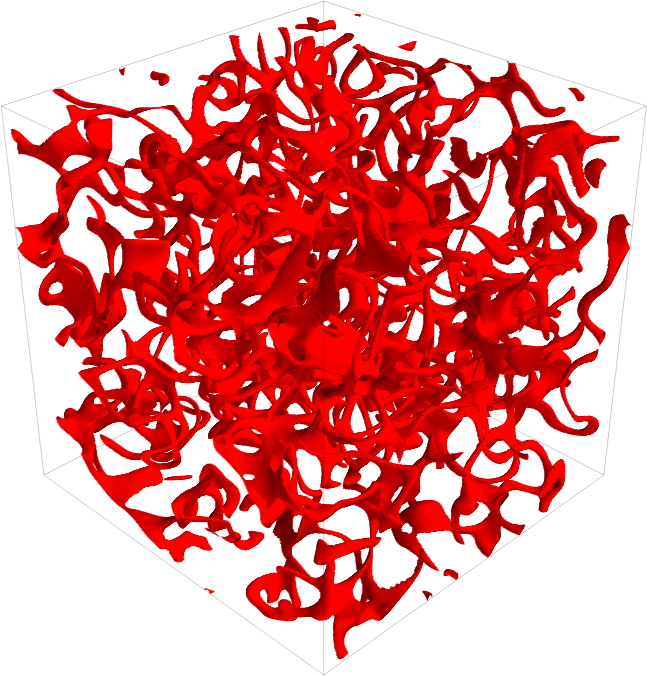
\includegraphics[width=0.25\linewidth]{nonequib/figures/IC/CF05-IC-t000}
    \raisebox{1.6in}{b)}~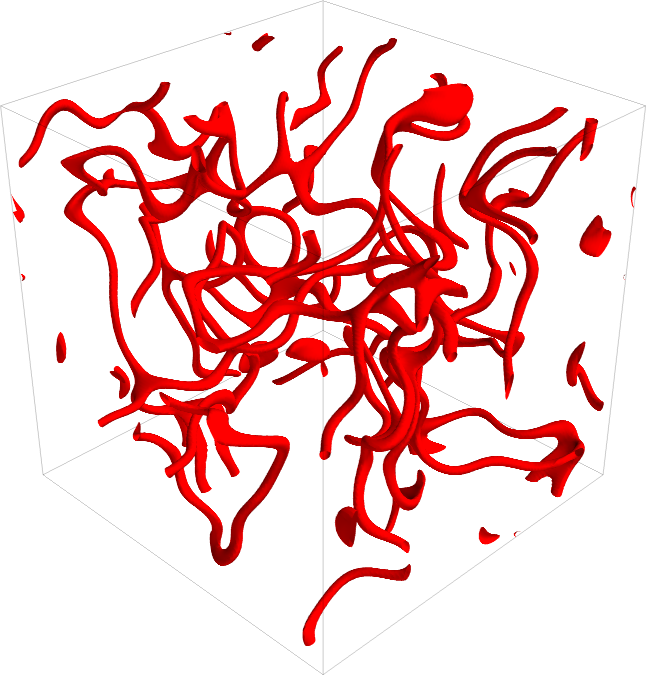
\includegraphics[width=0.25\linewidth]{nonequib/figures/IC/CF05-IC-t200}
    \raisebox{1.6in}{c)}~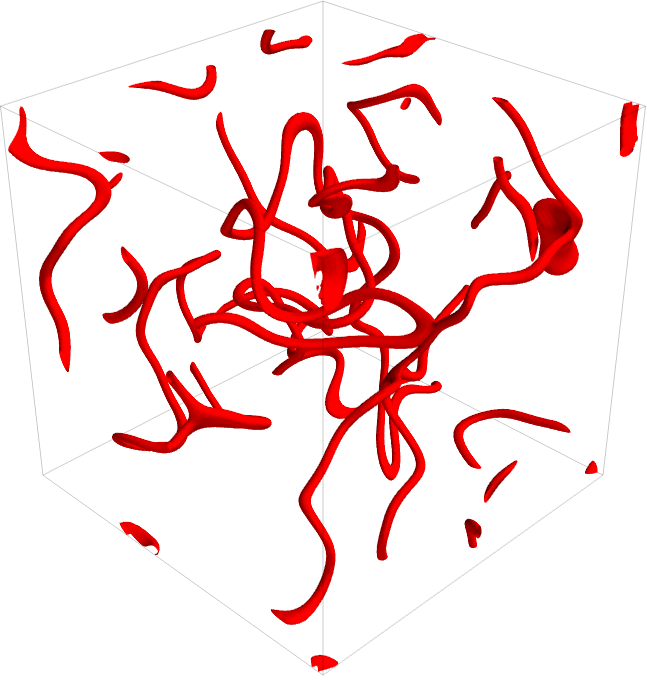
\includegraphics[width=0.25\linewidth]{nonequib/figures/IC/CF05-IC-t400}\\
    \raisebox{1.6in}{d)}~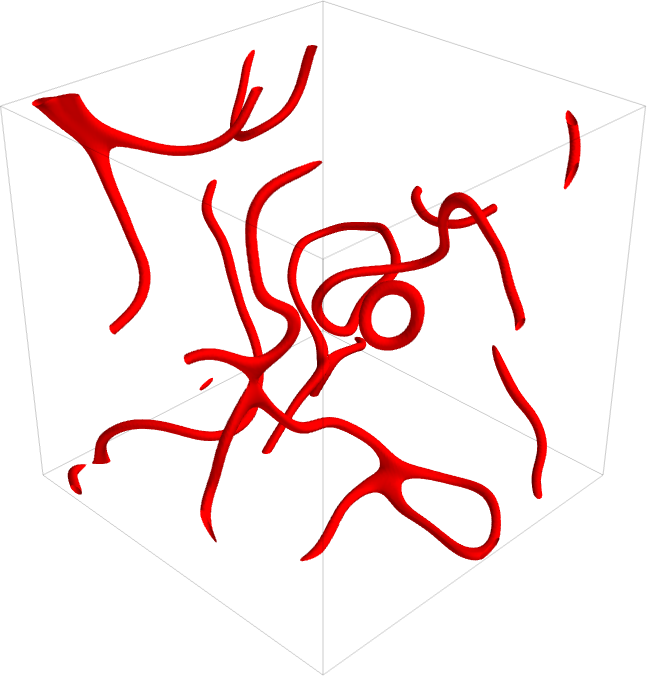
\includegraphics[width=0.25\linewidth]{nonequib/figures/IC/CF05-IC-t800}
    \raisebox{1.6in}{e)}~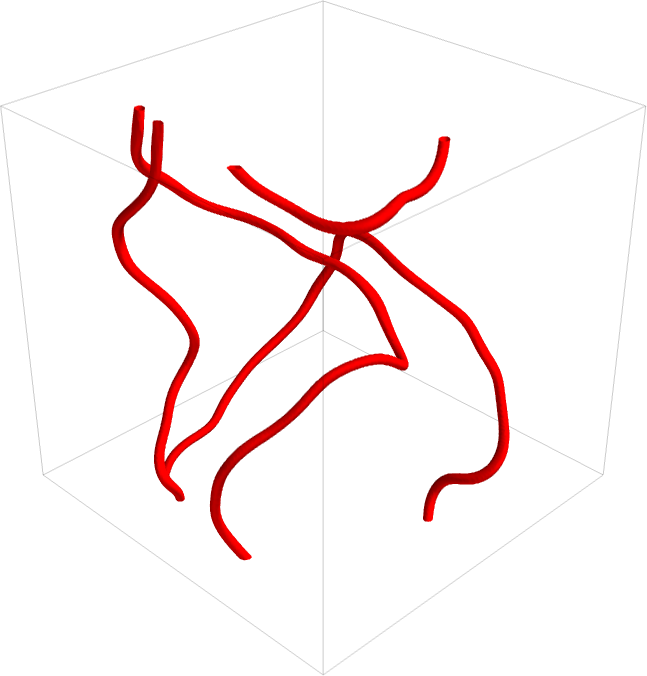
\includegraphics[width=0.25\linewidth]{nonequib/figures/IC/CF05-IC-t1600}
    \raisebox{1.6in}{f)}~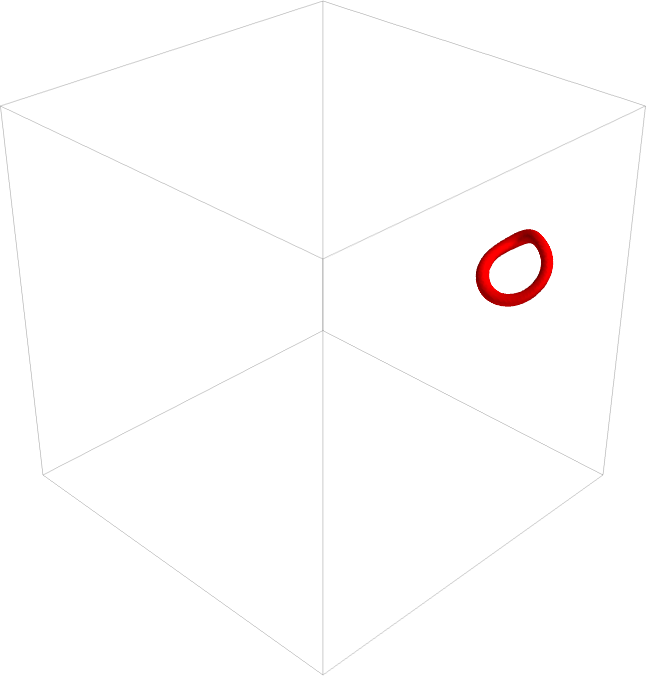
\includegraphics[width=0.25\linewidth]{nonequib/figures/IC/CF05-IC-t4000}
    \caption{A sample evolution of the turbulent vortex tangle present in the condensed part of the Bose gas as it decays to equilibrium. Here the final condensate fraction of the gas at equilibrium is $\rho_0/\rho = 0.48$. Shown are isosurfaces of the quasi-condensate density at isosurface level $0.05\braket{|\hat{\psi}|^2}$ at times (a) $t/\tau=0$, (b) $500$, (c) $1000$, (d) $2000$, (e) $4000$, and (f) $10\,000$. At later times (not shown) all vortex lines dissipate from the system.
}
    \label{fig:thermal}
\end{figure}

Its physical properties, e.g. temperature and condensate fraction, are uniquely determined by $N$ and the kinetic energy of the system~\cite{PhysRevLett.95.263901}.  The equilibrium state of the non-condensed particles follows the Rayleigh-Jeans distribution, modified by the nonlinear interaction with the condensed particles \cite{PhysRevLett.95.263901}.  It is interesting to note that the equilibrium condensate fraction is insensitive to the number of modes, providing that the number of modes is, or exceeds, $16^3$ modes.  This suggests that this number of modes is sufficient to model the thermodynamic limit of the system. For comparison, we employ $192^3$ modes.

The quasi-condensate wavefunction is used to visualise the condensed part of the Bose gas, using evolving isosurface levels of $|\hat{\psi}|^2 = 0.05\braket{|\hat{\psi}|^2}$. This level was chosen so that the resulting vortex structures are shown with approximately constant cross-sectional radius similar to the radius of a true vortex core (facilitated by the approximate quasi-condensate density term $\braket{|\hat{\psi}|^2}$).

\subsection{Approximate temperature of the gas}
\begin{figure}
\begin{center}
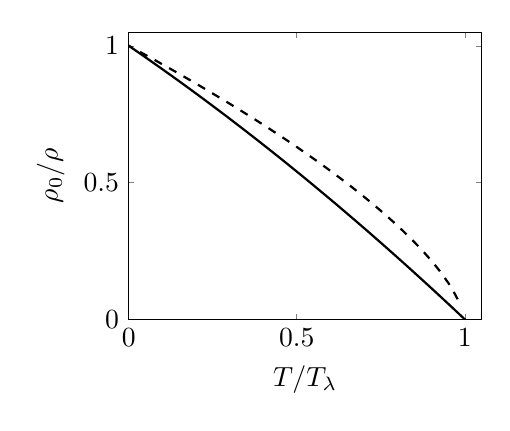
\begin{tikzpicture}
  \begin{axis}[samples=350,ylabel near ticks,xlabel near ticks,
      width=0.5\linewidth,
        xlabel=$T/T_\lambda$,
        ylabel=$\rho_0/\rho$,
        xmin=0,
        xmax=1.05,
        ymin=0,
        ymax=1.05,
        major tick length = 0.07cm]
    \addplot+[mark=none,color=black,thick] {1 - (1 - 0.2275*sqrt(0.5))*x - 0.2275*sqrt(0.5)*x^2};
    \addplot+[mark=none,color=black,dashed,thick] {(1 - x)^(2/3)};
  \end{axis}
\end{tikzpicture}%
\end{center}
\caption{\label{fig:cfvst}The condensate fraction and temperature relation for a weakly-interacting Bose gas for our simulation parameters (black solid line) and for an ideal non-interacting Bose gas (black dashed line).}
\end{figure} 

As we first saw in Section \ref{section:becinintro}, using the statistical mechanics of bosons it can be shown that for a {\it non-interacting} ideal gas of bosons there exists a simple prediction for how the condensate fraction of the gas grows as temperature decreases \cite{Pethick},
\begin{equation}
N_0 = N \left [ 1-\left ( \frac{T}{T_\lambda} \right )^\beta \right ],
\end{equation}
where $N_0$ is the number of condensed particles, $T_{\lambda}$ is the critical temperature for condensation and $\beta$ is a parameter that depends on the geometry of the system. For particles in a 3 dimensional box, $\beta=3/2$ \cite{Pethick}. By inverting this relation we could obtain a simple minded approximation for the temperature of our equilibrated Bose gas, ignoring interactions.

However, Berloff {\it et al.} \cite{berloff_2007} recently provided the following empirical relationship for a {\it weakly-interacting} Bose gas in a 3 dimensional box:
\begin{equation}
  \frac{T}{T_\lambda} = 1 - (1 - \alpha\sqrt{\rho})\frac{\rho_0}{\rho} - \alpha\sqrt{\rho}\,\left(\frac{\rho_0}{\rho}\right)^2,
  \label{eq:temp}
\end{equation}
where $\alpha=0.2275$ is a fitting parameter. We will use this relation throughout the chapter to evaluate the temperature of the gas using the condensate fraction at equilibrium. The relation is compared to the relation for an ideal non-interacting Bose gas in Figure \ref{fig:cfvst}. Table \ref{tbl:cond_frac} lists the resulting approximate temperatures at equilibrium for the parameters chosen in our simulations.

\subsection{Energy scales of the vortex tangle}


\begin{figure}
\centering
\begin{tikzpicture}
    \begin{axis}[ylabel near ticks,xlabel near ticks,
        width=0.6\linewidth,
        xlabel={},
        ylabel={},
        xmin=0.025,
        xmax=9,
        ymin=5e-5,
        ymax=10,
        major tick length = 0.00cm,
        minor tick length = 0.00cm,
    xmode=log,
    ymode=log,
    axis y line*=right,
        axis x line*=top,
        ytick={0},
        yticklabels={,,},
        xtick={0.043,0.1709,6.28},
        xticklabels={$k_D$, $k_\ell$, $k_\xi$} ]  
          \addplot+[mark=none,black!99,ultra thick,dashed,domain=1.3:3.45] {(3e-2)*x^(-3)};
      \addplot+[mark=none,black!99,ultra thick,dashed,domain=0.1:0.5] {(6e-1)*x^(-1)};    
          \addplot+[mark=none,black!50,dashed] coordinates {(6.28, 1e-5) (6.28, 10)};
      \addplot+[mark=none,black!50,dashed] coordinates {(0.043, 1e-5) (0.043, 10)};
      \addplot+[mark=none,black!50,dashed] coordinates {(0.1709, 1e-5) (0.1709, 10)};
    \end{axis}
    \begin{axis}[samples=200,ylabel near ticks,xlabel near ticks,
        width=0.6\linewidth,
        xtick pos=left,
        ytick pos=left,
        xlabel=$k \xi$,
        ylabel=$\hat{E}^i_{\rm kin}/\mu$,
        xmin=0.025,
        xmax=9,
        ymin=5e-5,
        ymax=10,
        axis y line*=left,
        axis x line*=bottom,
        major tick length = 0.1cm,
        minor tick length = 0.07cm,
    xmode=log,
    ymode=log,
    restrict expr to domain={x}{0.0001:4.5}]
      \addplot+[red,only marks,mark options={scale=0.5}] file {nonequib/kk_vs_Eikin-CF02-t300.dat};
      \addplot+[green,only marks,mark options={scale=0.5}] file {nonequib/kk_vs_Eikin-CF05-t300.dat};
      \addplot+[mark=diamond*,blue,only marks,mark options={scale=0.7}] file {nonequib/kk_vs_Eikin-CF075-t300.dat};
      \node at (axis cs: 3,0.004) {$k^{-3}$};
      \node at (axis cs: 0.25,5.5) {$k^{-1}$};
    \end{axis}
  \end{tikzpicture}
  \caption{\label{fig:spectra}Incompressible kinetic energy spectrum for the quasi-condensate tangles with $\rho_0/\rho=0.22$ (red circles), $\rho_0/\rho=0.48$ (green squares), and $\rho_0/\rho=0.77$ (blue diamonds) at time $t/\tau=300$. Dashed lines show the scale of the healing length, $k_\xi$, the length scale of inter-vortex spacing $k_\ell$, and the length scale of the periodic box $k_D$. Guide lines proportional to $k^{-3}$ and $k^{-1}$ are also shown. }
\end{figure}
One method to characterise the turbulence of the vortex tangle formed in the quasi-condensate is by studying how the kinetic energy of the vortices is distributed over length scales. There are three length scales of particular interest: the length scale associated with the computational box, the length scale associated with the superfluid healing length, and the length scale associated with the inter-vortex spacing, $\ell$. The corresponding wavenumbers are $k_D=2\pi/D$, $k_\xi = 2\pi/\xi$, and $k_\ell = 2\pi/\ell$. The inter-vortex spacing can be approximated by $1/\sqrt{L}$, a relation derived through dimensional arguments where $L$ is the vortex line-density (length of vortex line per unit volume). These length scales provide the perspective required to interpret the distribution of energy.

The kinetic energy of the quasi-condensate is defined as $E_{\rm kin} = \int\!\frac{\hbar^2}{2m}|\nabla\hat\psi|^2\,\mathrm{d}\mathbf{r}$.
 Using Parseval's theorem, the corresponding kinetic energy spectrum, $\hat{E}_{\rm kin}(k)$, can be written in terms of the angle-average of $\left |\mathcal{F}(\sqrt{E_{\rm kin}})\right |^2$ \cite{Nore},
where $\mathcal{F}$ denotes the Fourier transform, so that,
\begin{equation}
  \int E_{\rm kin}({\bf r})~{\rm d}^3{\bf r} = \int \hat{E}_{\rm kin}(k)~{\mathrm d}k.
  \label{eq:Ekin}
\end{equation}
The kinetic energy can be further decomposed into compressible and incompressible parts, $E_{\rm kin} = E^i_{\rm kin} + E^c_{\rm kin}$, by using the decomposition \cite{Nore} $\sqrt{n}v_j = (\sqrt{n}v_j)^c + (\sqrt{n}v_j)^i$, with $\nabla(\sqrt{n}v_j)^i=0$, where $n$ is the fluid density and $\mathbf{v}$ is the fluid velocity. The incompressible kinetic energy spectrum is then denoted $\hat{E}^i_{\rm kin}(k)$, defined similarly to $\hat{E}_{\rm kin}(k)$.

We calculate the incompressible energy spectrum of the quasi-condensate at various temperatures, sampled at time $t/\tau=300$ so as to characterise the vortex tangle before significant decay, while providing enough time for the quasi-condensate to form. The resulting spectra are shown in Figure \ref{fig:spectra}. Most of each spectrum demonstrates a $\sim k^{-3}$ scaling, corresponding to the vortex core on the scale of $k_\ell<k<k_\xi$. For quasi-classical turbulence, we would expect a build up of kinetic energy at scales larger than the inter-vortex distance, $k_D<k<k_\ell$, demonstrating the famous Kolmogorov $k^{-5/3}$ power law scaling. In our simulations the incompressible kinetic energy spectrum does {\it not} show a definitive $k^{-5/3}$ scaling. The spectra instead show a marked lack of energy build up at scales $k_D<k<k_\ell$. In contrast to quasi-classical turbulence, ultra-quantum turbulence predicts a $k^{-1}$ scaling at scales $k_D<k<k_\ell$. A guide line proportional to this power law is shown Figure \ref{fig:spectra}.

\section{Relaxation of the vortex tangle}
\begin{figure}
\hspace*{1cm}(a)\hspace{7cm}(b)\hspace{3cm}
\begin{center}
\begin{tikzpicture}
  \begin{axis}[samples=200,ylabel near ticks,xlabel near ticks,
      width=0.45\linewidth,
      xtick pos=left,
      ytick pos=left,
      xlabel=$t/\tau$,
      ylabel=$L\xi^2$,
      xmin=10,
      xmax=15000,
      ymin=1.5e-5,
      ymax=3e-3,
      major tick length = 0.1cm,
      minor tick length = 0.07cm,
      xmode=log,
      ymode=log]
      \addplot+[mark=diamond*,blue,only marks,mark options={fill=blue}] table[x=t,y=l] {nonequib/l_vs_t_CF075.dat};
      \addplot+[green,only marks,mark=square*,mark options={fill=green,scale=0.7}] table[x=t,y=l] {nonequib/l_vs_t_CF05.dat};
      \addplot+[red,only marks,mark=*,mark options={fill=red,scale=0.7}] table[x=t,y=l] {nonequib/l_vs_t_CF02.dat};
      \addplot+[mark=none,black,ultra thick,dashed,domain=600:3000] {(6e-1)*x^(-1)};
      \node at (axis cs: 2000,6e-4) {$t^{-1}$};
  \end{axis}
\end{tikzpicture}
\begin{tikzpicture}
    \begin{axis}[samples=200,ylabel near ticks,xlabel near ticks,
      width=0.45\linewidth,
      ylabel near ticks,
      xlabel near ticks,
      xtick pos=left,
      ytick pos=left,
      ylabel={$\rho_0/\rho$},
      xlabel={$t/\tau$},
      xmin=0,
      xmax=5000,
      ymin=0,
      ymax=1.1]
      \addplot+[red,mark=none,ultra thick] file {nonequib/cf_vs_t_CF02.dat};
      \addplot+[green,mark=none,ultra thick,dashed] file {nonequib/cf_vs_t_CF05.dat};
      \addplot+[blue,mark=none,ultra thick,dash pattern=on 4pt off 1pt on 1pt off 1pt] file {nonequib/cf_vs_t_CF075.dat};
    \end{axis}
\end{tikzpicture}
\end{center}
\caption{\label{fig:ll_t} (a) Vortex line density over time for $\rho/\rho_0=0.22$ (red circles), $\rho/\rho_0=0.48$ (green sqaures), and $\rho/\rho_0=0.77$ (blue diamonds). Each line is an average of 5 simulations. A line proportional to $t^{-1}$, characteristic of the decay of a ultra-quantum turbulence, is shown (dashed black line) as reference. (b) Condensate fraction over time for equilibrium states with $\rho/\rho_0=0.22$ (red solid line), $\rho/\rho_0=0.48$ (green dashed line), and $\rho/\rho_0=0.77$ (blue dot-dashed line). }
\end{figure}
As the condensate evolves over the course of the simulation, the initially-formed dense vortex tangle remains random and isotropic throughout the decay to one or more vortex rings, which eventually also decay, leading to a vortex-free state (the ``equilibrated" state). A example of such a decay is shown in Figure \ref{fig:thermal}.

Insight into the nature of the quasi-condensate turbulence can be obtained by investigating the relaxation of the vortex tangle, obtained by monitoring the vortex line-density $L$. We estimate the vortex line-length from the total volume of the isosurface tubes, $V_{\rm t}$. We assume that each vortex tube has uniform constant circular cross-sectional area $A_{\rm t}$; the total vortex line-length is then $V_{\rm t}/A_{\rm t}$.

Note that this approximation is only strictly valid for vortices well separated in space and for steady condensate fraction (so that the healing length of the quasi-condensate is constant). A more sophisticated and robust algorithm for calculating and tracking vortex line length has recently been described \cite{Kerr14,Villois16}, however the computational requirements are higher. We find that the computationally efficient estimate we employ here is accurate enough for our analysis due to the fact that it is only at very early times where the condensate fraction changes significantly [Figure \ref{fig:ll_t}(b)], and our vortices are indeed well separated for the majority of the decay [Figure \ref{fig:thermal}(b-f)].

\begin{table}
\centering
\begin{tabular}{ccc}
{\it $\rho_0/\rho$} & {\it Power law fit} & {\it $95\%$ confidence interval} \\
\hline \\ [-2ex]
$0.22$ & $-1.04$ & $(-1.10, -0.98)$\\
$0.48$ & $-0.95$ & $(-1.01, -0.89)$\\
$0.77$ & $-0.81$ & $(-0.89, -0.72)$\\
\hline
\end{tabular}
\caption{The resulting value of $b$ for fitting the decay of the vortex line density over time to the equation $f(t) = at^b+c$ for the data demonstrated in Figure \ref{fig:ll_t}, including a $95\%$ confidence interval.}
\label{tbl:fits}
\end{table}

The decay of the vortex line density is shown in Figure \ref{fig:ll_t}. When the condensate fraction at the simulated value of $\rho_0/\rho = 0.22$, the decay of $L$ is in good agreement with the predicted ultra-quantum decay of $L(t) \propto t^{-1}$ \cite{WalmsleyGolov2008}. Our lowest temperature simulations show a deviation from the $t^{-1}$ decay law, suggesting a shift to longer vortex tangle decay times as the gas is simulated closer to the zero temperature limit. The decays are quantitatively compared to the predicted power law in Table \ref{tbl:fits}, showing a power law best fit and $95\%$ confidence interval.

The velocity correlation function, $f(r)$, is defined at a fixed point in time as
\begin{equation}
f(r) = \frac{\langle v_x({\bf r})v_x({\bf r} +  r\hat{\bf e}_x) \rangle}{\langle v_x({\bf r})^2 \rangle}
\end{equation}
where $\mathbf{v}$ is the quasi-condensate fluid velocity and the ensemble average is performed over positions ${\bf r}$. While we have used the $x$ direction in the definition of $f(r)$, due to the isotropic nature of the turbulence using the $y$ or $z$ direction leads to similar results. The function is a dimensionless measure of velocity correlation at distance $r$, with $f(0)=1$, and is shown in Figure \ref{fig:IS_t} (a) for the three of our simulated parameter sets (spanning the range of temperatures) at a time of $t/\tau = 300$. The choice of time allows us to probe the velocity correlations after the quasi-condensate has formed, but before any significant decay of the vortex tangle has taken place. For the time chosen, the velocity correlation functions are not significantly different for each of our simulation parameters. The value of $f(r)$ smoothly drops to approximately $0$ at around $r/\xi = 20$. Short scale correlation is expected due to the structure of the fluid velocity around a vortex core. The lack of velocity correlation at large scales suggests a lack of vortex bundles (collections of co-rotating aligned vortex lines of the same circulation), theorised to be the driving force of the large scale kinetic energy in quasi-classical turbulence.

The integral scale provides a convenient measure of the distance over which velocities are correlated by producing a scalar value from the velocity correlation function. It is defined as
\begin{equation}
I = \int\limits_0^\infty\! f(r)\, \mathrm{d}r,
\end{equation}
and is shown in Figure \ref{fig:IS_t} (b) evolving over time during the vortex tangle evolution. Three lines corresponding to different temperatures are shown, with each line an average of 5 simulations. The value of $I$ increases as the vortex tangle decays in all of the simulated cases, an expected result as vortices decay and so velocity becomes correlated over larger regions of space. At early times, $I(0)\approx0$, reflecting the random nature of the initial tangle. As the tangle decays, the value of $I$ grows, but remains significantly less than $\ell$, demonstrating that as the vortex tangle evolves over time, there is no evidence of vortex lines ``bundling up'' to create a large scale flow.

\begin{figure}
\hspace*{1cm}(a)\hspace{7cm}(b)\hspace{3cm}
\begin{center}
\begin{tikzpicture}
  \begin{axis}[samples=200,ylabel near ticks,xlabel near ticks,
        width=0.45\linewidth,
        xtick pos=left,
        ytick pos=left,
        xlabel={$r/\xi$},
        ylabel={$f$},
        xmin=0,
        xmax=20,
        ymin=-0.1,
        ymax=1.1,
        major tick length = 0.1cm,
        minor tick length = 0.07cm]
      \addplot+[red,mark=none,ultra thick] file {nonequib/f_vs_r_CF02.dat};
      \addplot+[green,mark=none,ultra thick,dashed] file {nonequib/f_vs_r_CF05.dat};
      \addplot+[blue,mark=none,ultra thick,dash pattern=on 4pt off 1pt on 1pt off 1pt] file {nonequib/f_vs_r_CF075.dat};
    \end{axis}
  \end{tikzpicture}
\begin{tikzpicture}
    \begin{axis}[samples=200,ylabel near ticks,xlabel near ticks,
    width=0.45\linewidth,
    ylabel near ticks,
    xlabel near ticks,
    xtick pos=left,
        ytick pos=left,
        ylabel={$I/\xi$},
        xlabel={$t/\tau$},
        xmin=0,
        xmax=4500,
        ymin=0,
        ymax=150]
      \addplot+[red,mark=*,thick,mark options={fill=red}] file {nonequib/IS_vs_t_CF02.dat};
      \addplot+[green,mark=square*,thick,mark options={fill=green,scale=0.7}] file {nonequib/IS_vs_t_CF05.dat};
      \addplot+[blue,mark=diamond*,thick,mark options={fill=blue}] file {nonequib/IS_vs_t_CF075.dat};
      \addplot+[black,thick,mark=none,dashed] table[x expr=\thisrow{t}, y expr=1/sqrt(\thisrow{l})] {nonequib/l_vs_t_CF02.dat};
    \end{axis}
  \end{tikzpicture}
  \end{center}
  \caption{\label{fig:IS_t}(a) Snapshots of the velocity correlation function $f(r)$ at time $t = 300\tau$ for equilibrium states with $\rho/\rho_0=0.22$ (red solid line), $\rho/\rho_0=0.48$ (green dashed line), and $\rho/\rho_0=0.77$ (blue dot-dashed line). (b) The integral scale as the quasi-condensate vortex tangle decays, for equilibrium states with $\rho/\rho_0=0.22$ (red circles), $\rho/\rho_0=0.48$ (green squares), and $\rho/\rho_0=0.77$ (blue diamonds). Also shown is the estimated inter-vortex spacing $\ell = 1/\sqrt{L(t)}$ for $\rho/\rho_0=0.22$ (dashed line).}
\end{figure}

The results of the velocity correlation and integral scale measurements confirm the conclusions of the kinetic energy spectrum measurements, that is, there is no evidence of energy at scales larger than the inter-vortex spacing at any point during vortex decay, at all simulated temperatures. This is perhaps not such a surprising result, the initial vortex tangle is seeded and forms from random fluctuations in the phase of the 3D wavefunction, favouring the random nature of quasi-classical turbulence.


\section{Moving obstacle at finite-temperature\label{sec:obstacle}}
\subsection{Critical velocity for vortex nucleation}
Having obtained the equilibrated finite-temperature states of the Bose gas, we now move on to consider a laser-induced obstacle moving through the gas.  The obstacle, uniform in $z$, is translated in the $x$-direction at speed $v$.  Our simulations are conducted moving with the obstacle, transformed into the moving frame as in Section \ref{section:linearmovframe}. The obstacle is imposed through a time-independent cylindrical Gaussian potential, as described in Section \ref{section:3dcylinderpotential},
\begin{equation*}
  V({\bf r}) = V_0 \exp\left ( -\frac{x^2+y^2}{d^2}\right ),
\end{equation*}
where $d$ and $V_0$ parametrise the width and amplitude of the potential. The amplitude is linearly increased from $V_0 = 0$ at first introduction to its maximal value $V_0=5\mu$ over a period of $200\tau$.   The frame speed is increased adiabatically to the required value according to the temporal profile $v \tanh(\hat{t}/200 \tau)$, where $\hat{t}$ denotes the time from introduction of the obstacle.

Simulations are repeated (from identical initial conditions) with increasing terminal speeds (in steps of $0.057c$) until vortices are detected.  Vortex detection is by visual inspection of the filtered density, up to a maximum simulation time $\hat{t}=500\tau$ (which is long enough to ensure that the obstacle is fully introduced and at terminal speed, but otherwise arbitrary). This procedure defines the critical velocity $v_c$.  There is a systematic uncertainty in our measurement of $v_c$, arising from the discrete terminal speeds employed.  Note that we have repeated this process for multiple randomized initial conditions, and find no change in our measurement of $v_c$; that is, the systematic uncertainty due to using discretised speeds is larger than the statistical uncertainty arising from different random initial conditions.

\begin{figure}
\hspace*{1cm}(a)\hspace{7cm}(b)\hspace{3cm}
\begin{center}
  \begin{tikzpicture}
  \begin{axis}[samples=200,ylabel near ticks,xlabel near ticks,
        width=0.45\linewidth,
        xtick pos=left,
        ytick pos=left,
        xlabel=$\rho_0/\rho$,
        ylabel=$v_c/c$,
        xmin=0,
        xmax=1.1,
        ymin=0,
        ymax=0.55,
        major tick length = 0.07cm
      ]
      \addplot+[only marks,mark options={blue},error bars/error bar style={blue},  error bars/.cd,y dir=both,y explicit] table[x=cf,y=2xi,y error=2err] {nonequib/cf_vs_vc.dat};
      \addplot+[only marks,mark=square*,mark options={red},error bars/error bar style={red},  error bars/.cd,y dir=both,y explicit] table[x=cf,y=5xi,y error=5err] {nonequib/cf_vs_vc.dat};
      \addplot+[mark=none,color=black!50,thick,dashed] [domain=0:1.5] {0.46*sqrt(x)};
      \addplot+[mark=none,color=black!50,thick,dashed] [domain=0:1.5] {0.35*sqrt(x)};
    \end{axis}
    \begin{axis}[ylabel near ticks,xlabel near ticks,
        width=0.45\linewidth,
        xlabel=$T/T_\lambda$,
        ylabel={},
        xmin=0,
        xmax=1.1,
        ymin=0,
        ymax=1,
        major tick length = 0.07cm,
        axis y line*=right,
        axis x line*=top,
        yticklabels={,,},
        ytick={0},
        xtick={0,0.23,0.44,0.64,0.82,1},
        xticklabels={$1$, $0.8$, $0.6$, $0.4$, $0.2$,$0$}
        ]
    \end{axis}
  \end{tikzpicture}%
  \begin{tikzpicture}%
  \begin{axis}[samples=200,ylabel near ticks,xlabel near ticks,
        width=0.45\linewidth,
        xtick pos=left,
        ytick pos=left,
        xlabel=$d/\xi$,
        ylabel=$v_c/c$,
        xmin=0,
        xmax=23,
        ymin=0.17,
        ymax=0.35,
        major tick length = 0.07cm
      ]
      \addplot+[only marks,mark options={blue},error bars/error bar style={blue},  error bars/.cd,y dir=both,y explicit] table[x=d,y=vc,y error=err] {nonequib/d_vs_vc.dat};
      \addplot+[mark=none,color=black!50,thick,dashed] [domain=0:30] {0.26/x+0.18};
    \end{axis}
  \end{tikzpicture}
\end{center}
  \caption{\label{fig:vc-n0}(a) Critical velocity $v_{\rm c}$ for the moving Gaussian-shaped obstacle (uniform in $z$) as a function of condensate fraction $\rho_0/\rho$ and temperature $T/T_\lambda$, for obstacle widths $d=2\xi$ (blue circles) and $d=5\xi$ (red squares). The dotted lines show the analytic model $v_{\rm c}=\beta \sqrt{\rho_0/\rho}$ with fitted coefficients $\beta=0.46c$ and $0.35c$. (b) The critical velocity approaches an asymptotic value as the obstacle size is increased. Included is a fit of the form $v_{\rm c}=\alpha/d+\gamma$ with $\alpha=0.26~(\xi^2/\tau)$ and $\gamma=0.18 c$.  Errors bars represent the systematic uncertainty in $v_c$ due to the discretised values of $v$ considered.}
\end{figure}

Figure \ref{fig:vc-n0} (a) shows the variation of $v_c$ with both condensate fraction $\rho_0/\rho$ (lower abscissa) and temperature $T/T_\lambda$ (upper abscissa), for two example obstacles widths.  The critical velocity has a maximum value at zero temperature (unit condensate fraction), and decreases nonlinearly as temperature increases (condensate fraction decreases), reaching zero at the critical point for condensation.

At zero temperature, the critical velocity is of the order of the condensate speed of sound $c=\sqrt{\rho g/m}$, with a general form $v_{\rm c}(T=0)=\beta c$,
where $\beta$ is a parameter which depends solely on the shape of the
obstacle (here $d$ and $V_0$).  The simulated $v_c$ data in
Figure \ref{fig:vc-n0} closely follow the simple functional form
$v_{\rm c}(T) = v_{\rm c}(0) \sqrt{\rho_0/\rho}$, as shown by the dashed lines.
An expression for the critical velocity valid at zero and non-zero
temperatures is
\begin{equation}
v_{\rm c}(T)=\beta \sqrt{\rho_0 g/m}.
\label{eqn:finite_vc}
\end{equation}
In other words, for a given obstacle, the critical velocity is a fixed
fraction of the speed of sound based on the {\it condensate} density
rather than the total particle density \cite{leadbeater_2003}.

Figure \ref{fig:vc-n0} (b) shows the variation of $v_{\rm c}$ with the obstacle width $d$ at finite temperature, for the example of $T/T_\lambda =0.56$.   The qualitative behaviour is consistent with that seen in Chapter \ref{cha:wake} at zero temperature \cite{huepe00,rica2001,stagg_parker_14}: for small $d$ the critical velocity is sensitive to $d$ (due to the prominence of boundary effects) but as $d$ increases $v_c$ decreases towards a limiting value (the Eulerian limit).  However, the critical velocities are systematically reduced compared to the zero temperature case due to the reduced condensate speed of sound at finite temperature.


\subsection{Vortex nucleation pattern}
Finally we examine the manner in which vortices are nucleated from the obstacle.  At zero temperature, one expects the nucleation of straight anti-parallel vortex lines from the obstacle, either released in unison or staggered in time \cite{frisch92,saito10,stagg_parker_14}, which move downstream relative to the obstacle.  At finite temperature, we observe the loss of vortex symmetry along the obstacle axis, and three general regimes of vortex nucleation, with representative examples shown in Figure  \ref{fig:vort-lines}:

\begin{figure}
    %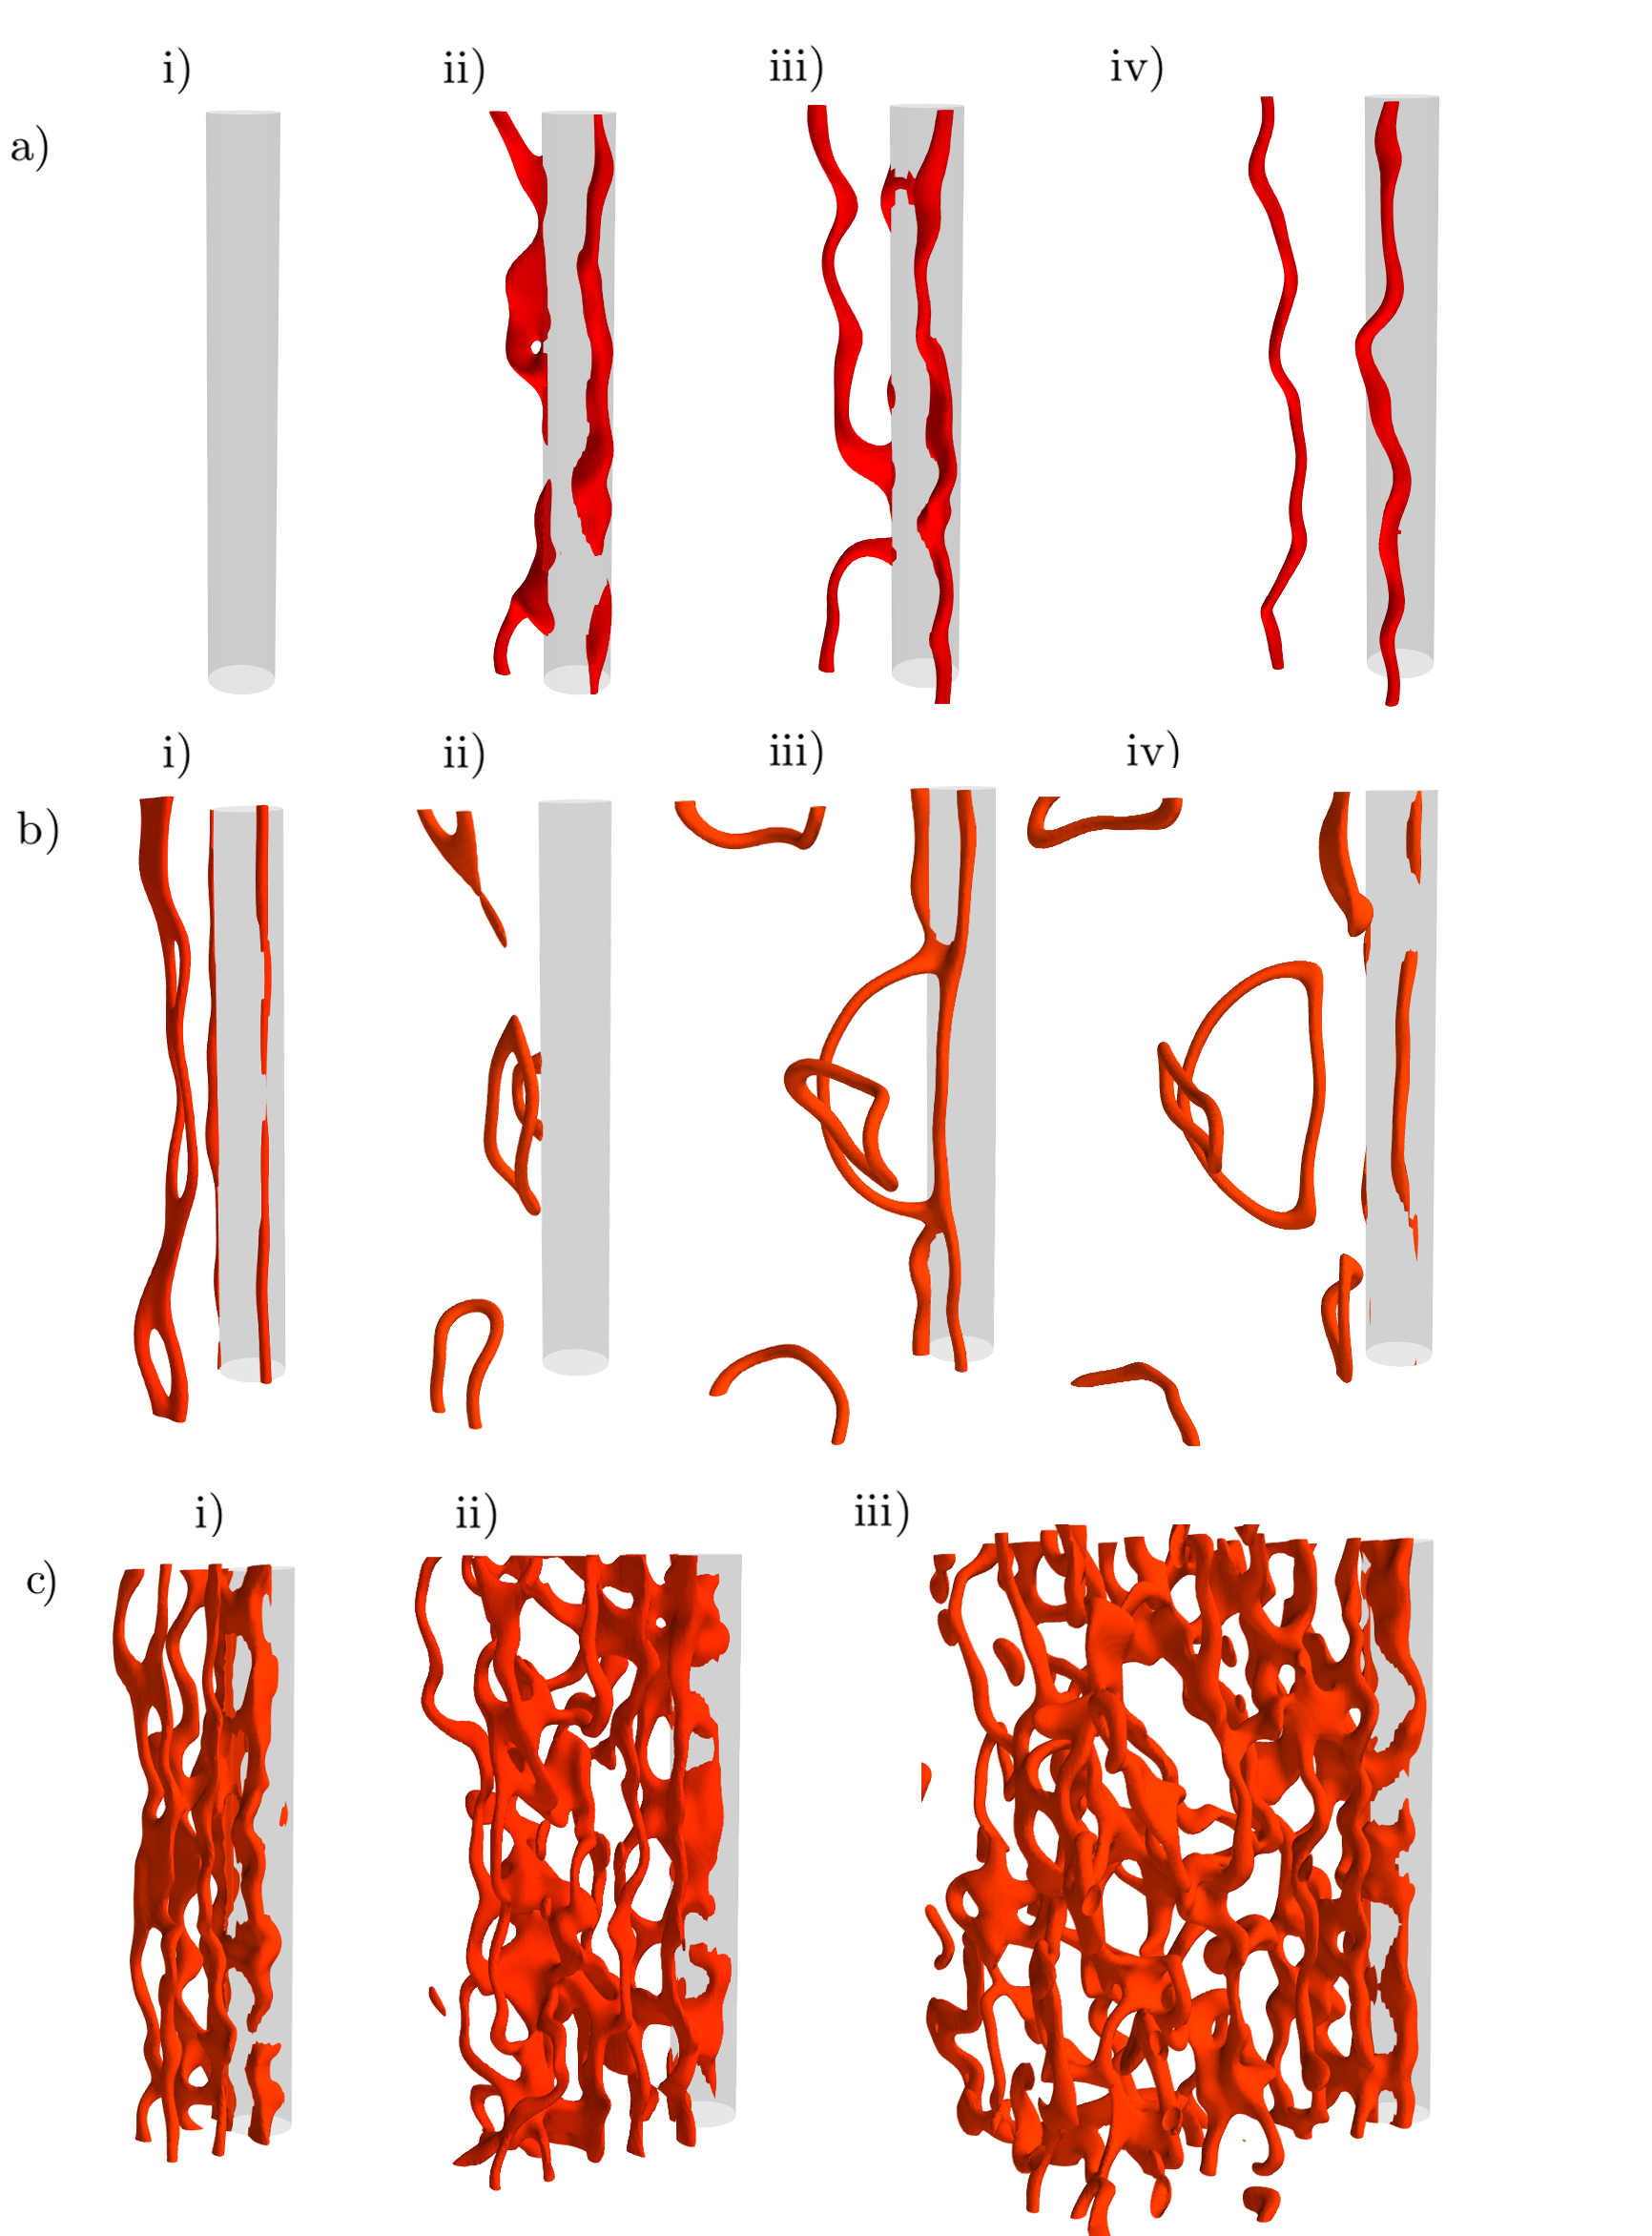
\includegraphics[width=0.9\linewidth]{nonequib/figures/vort}
    \centering
    \begin{tikzpicture}
      \node[anchor=south west] at (0,0) (image1) {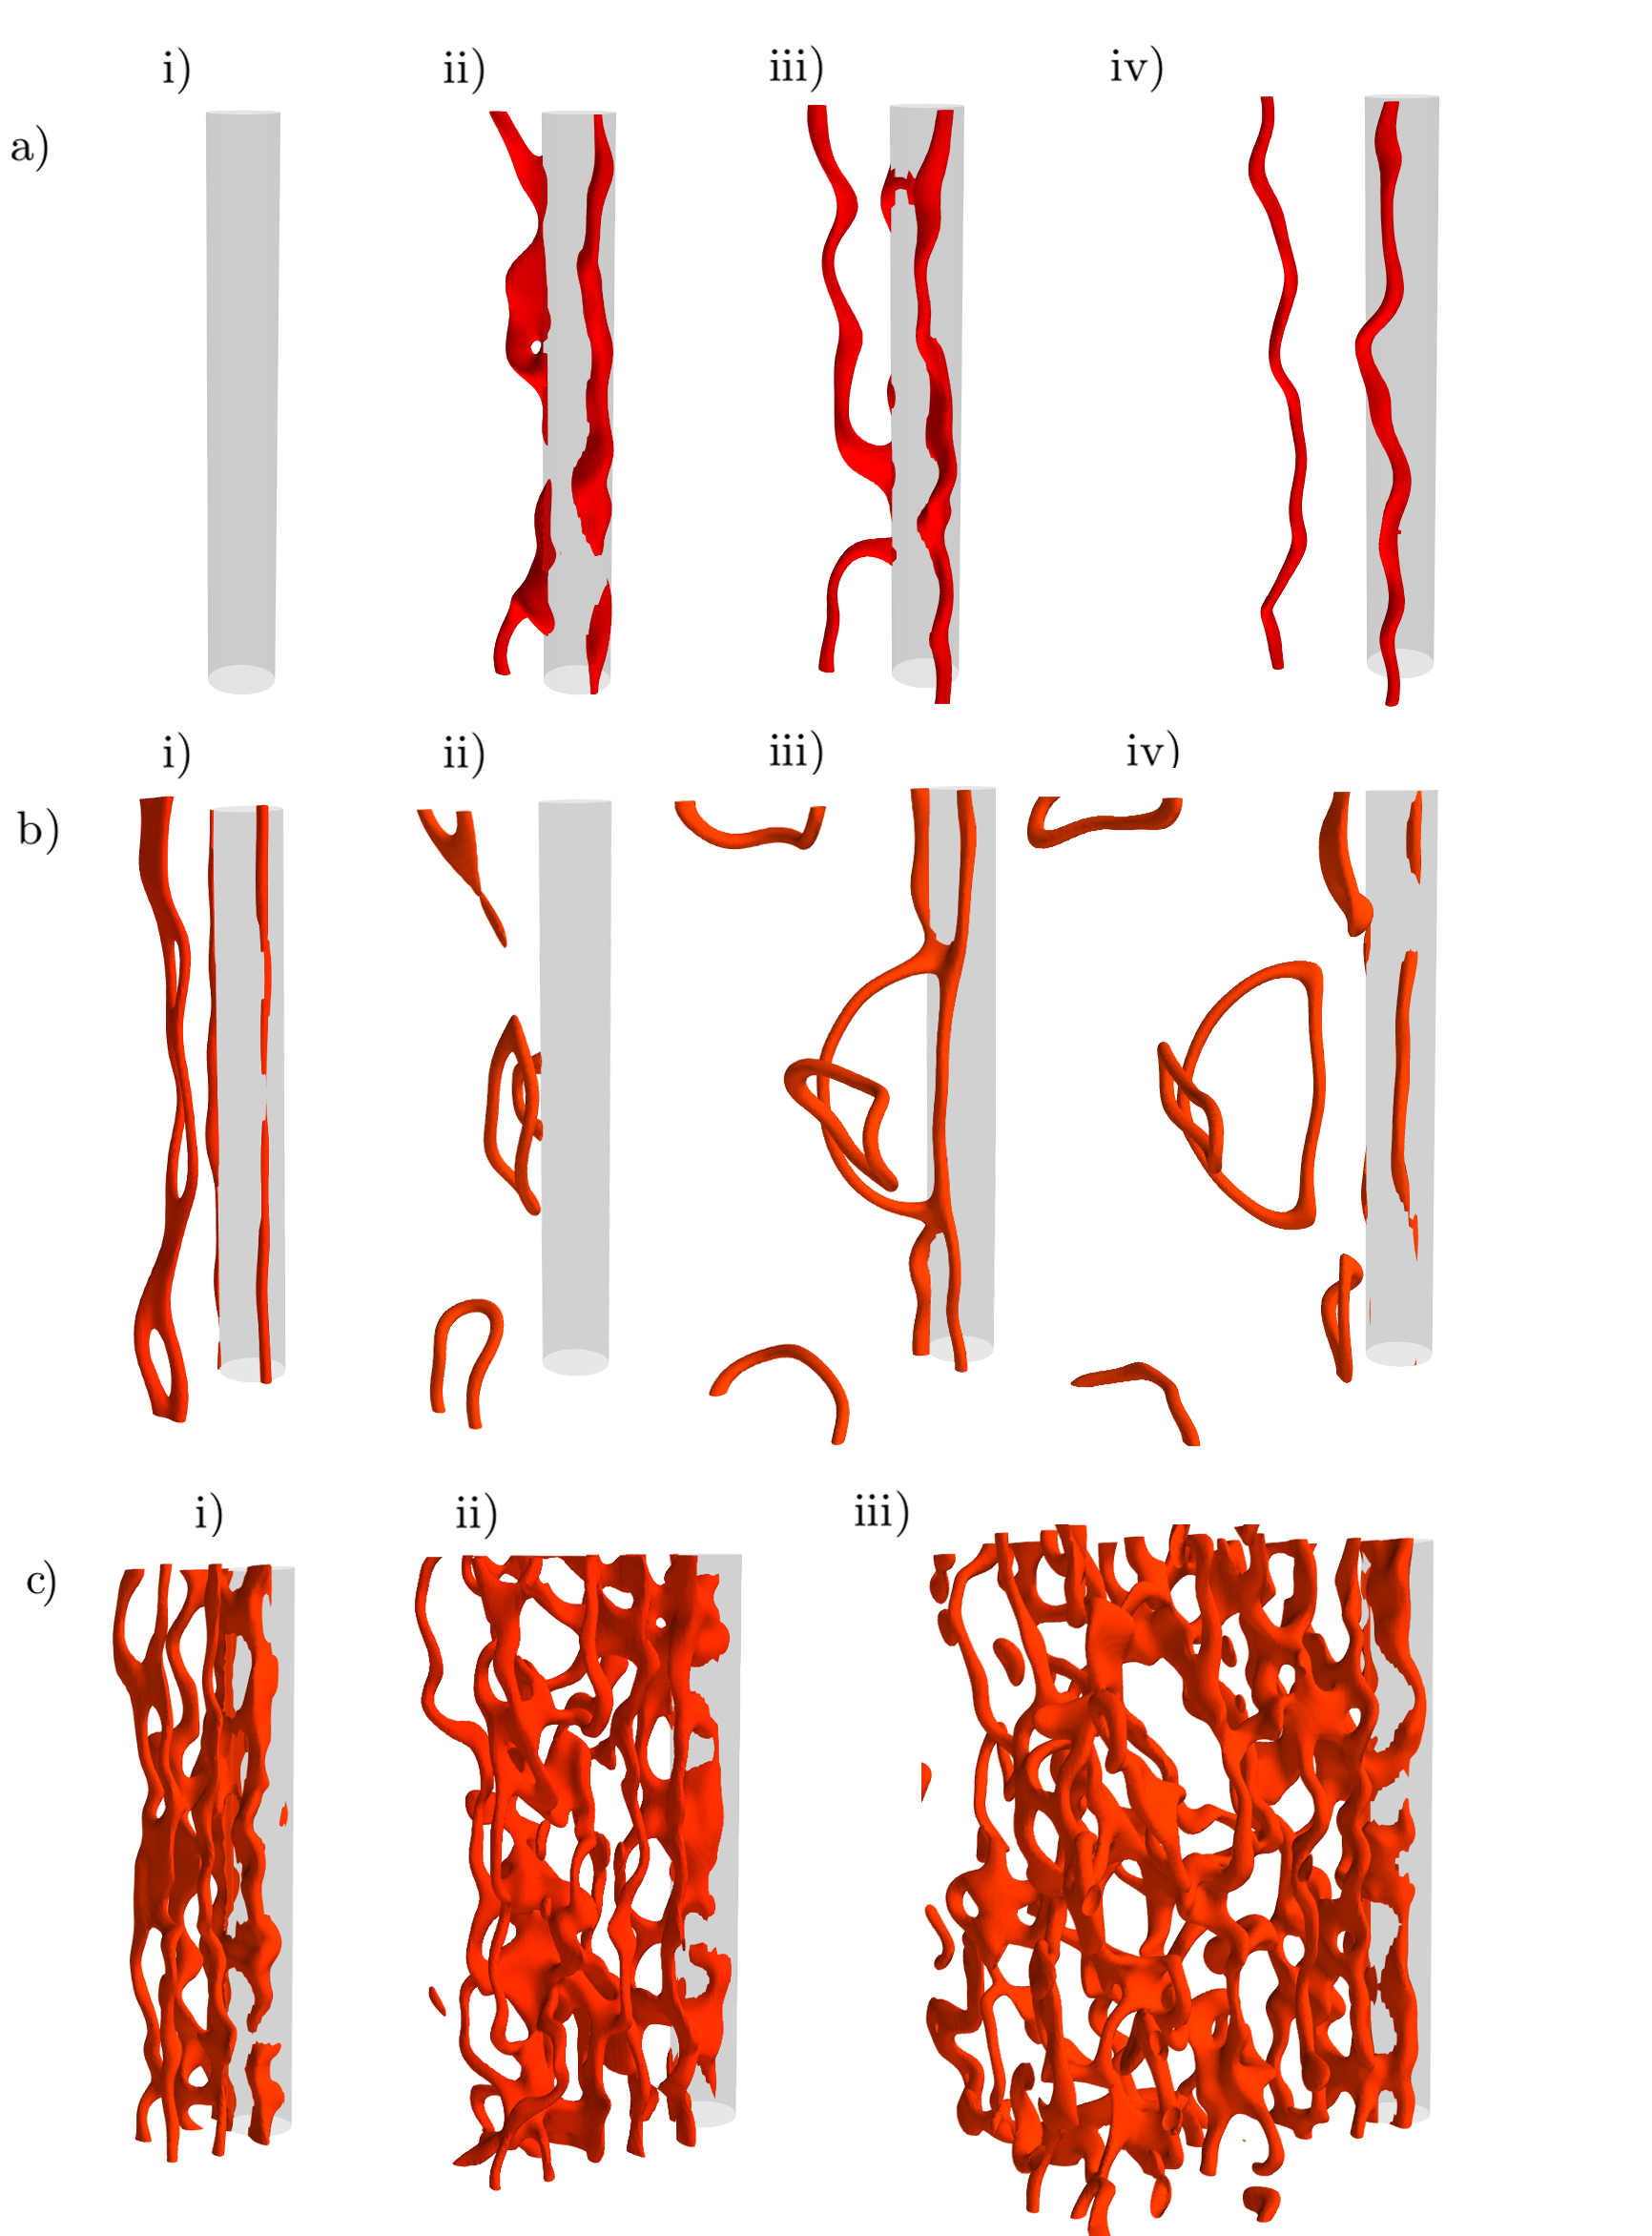
\includegraphics[width=0.9\linewidth]{nonequib/figures/vort}};
      \begin{scope}[x={(image1.south east)},y={(image1.north west)}]
      \node at (0.1,0.96) {i)};
      \node at (0.27,0.96) {ii)};
      \node at (0.46,0.96) {iii)};
      \node at (0.65,0.96) {iv)};

      \node at (0.1,0.66) {i)};
      \node at (0.27,0.66) {ii)};
      \node at (0.46,0.66) {iii)};
      \node at (0.65,0.66) {iv)};

      \node at (0.1,0.33) {i)};
      \node at (0.27,0.33) {ii)};
      \node at (0.56,0.33) {iii)};

      \node at (0.05,0.93) {a)};
      \node at (0.05,0.63) {b)};
      \node at (0.05,0.3) {c)};
      \end{scope}
    \end{tikzpicture}
    \caption{\label{fig:vort-lines} Snapshots of the typical vortex nucleation from the moving Gaussian-shaped obstacle with $d=5\xi$ (gray) in the finite temperature Bose gas. The three cases (a-c) are representative of the behaviour across the whole parameter space. Shown are  isosurfaces of the quasi-condensate density ($|\hat{\psi}|^2 = 0.05\braket{|\hat{\psi}|^2}$).  (a) Vortices are shed as pairs of anti-parallel vortex lines.  Here the system parameters are $\rho_0/\rho = 0.22$ and $v=0.17c$, and the snapshots correspond to times (i) $\hat{t}/\tau=210$, (ii) $460$, (iii) $585$ and (iv) $710$.  (b) Vortex rings are nucleated from the obstacle.  The system parameters are $\rho_0/\rho = 0.91$ and $v=0.42c$, and the times are (i) $\hat{t}/\tau=500$, (ii) $700$, (iii) $875$ and (iv) $950$. (c) A vortex tangle forms behind the obstacle. The system parameters are $\rho_0/\rho = 0.35$ and $v=0.59c$, and the times are (i) $\hat{t}/\tau=250$, (ii) $375$ and (iii) $500$. }
\end{figure}


\begin{description}
\item[Vortex lines] A pair of ``wiggly'' vortex lines is produced  [Figure  \ref{fig:vort-lines}(a)].  The wiggles are driven by the thermal fluctuations, which cause the vortex elements to be nucleated at slightly different times along the obstacle; this is visible at intermediate times (snapshots (iii) and (iv)).   These elements ultimately merge together along the axis of the obstacle to form a wiggly vortex/anti-vortex line. Similar vortex configurations
in the form of lines which are partially attached to a thin wire 
were also observed in liquid helium \cite{zieve2001}. 
\item[Vortex rings]  Here vortices predominately form vortex
rings [Figure \ref{fig:vort-lines}(b)].  The vortex loops generated
at the obstacle rapidly peel away from the obstacle, reconnecting with
adjacent loops to form rings. Due to the way the vortex rings form initially along the obstacle, they are elliptical and polarised such that they are longer along the obstacle axis. 
\item[Vortex tangle]  Strong
interaction between successively nucleated vortices leads to the formation of a complex tangle of vortex lines behind the obstacle [Figure \ref{fig:vort-lines}(c)].
\end{description}

While the vortex line regime is analogous to the zero temperature case, no analogue occurs for the ring and tangle regimes.   We note that even a small amount of thermal fluctuations is enough to vastly change the form of vortex nucleation, such as the vortex rings produced in Figure \ref{fig:vort-lines}(c) for a condensate fraction of $0.91$.

To systematically map the occurrence of these regimes, we measure the vortex line-density $L$ and vortex polarity $R$ (described below) at a fixed observation time of $\hat{t}=500\tau$, throughout the parameter space of flow velocity and condensate fraction.  The results are presented in Figure \ref{fig:vort-vals}.  Below the critical velocity (solid black line) no vortices are produced, and thus $L=0$.  Above the critical velocity, $L$ increases strongly with the flow velocity.  This is to be expected since the frequency of vortex nucleation increases with flow velocity \cite{frisch92}.  $L$ also increases with decreasing condensate fraction (increasing temperature), indicating the significant role of thermal fluctuations in enhancing vortex production.

Just above the critical velocity, where the vortex line-length density is relatively small, vortex nucleation occurs through vortex lines and rings.  The low flow velocity ensures that the vortex nucleation frequency is low, thereby suppressing strong interaction or reconnection between nucleated vortices.  Here, whether lines or rings are produced is sensitive to the random initial conditions, and so it is not possible to further distinguish these nucleation regimes within this parameter space. In these cases a more consistent characterisation of the vortex form is given by $R$, described below.   At higher flow velocities, where the vortex line-length density is relatively high, the nucleation frequency becomes sufficiently high that vortices immediately undergo strong interactions with each other, reconnecting and developing into a vortex tangle.  The transition in the parameter space from vortex lines/rings to tangles is indicated approximately by the dashed line, although statistical effects blur the true boundary.

\begin{figure}
  \centering
  \begin{tikzpicture}
    \begin{axis}[ylabel near ticks,xlabel near ticks,
        axis on top,
        width=0.5\linewidth,
        height=0.475\linewidth,
        xlabel=$\rho_0/\rho$,
        ylabel=$v/c$,
        xmin = 0,
        xmax = 1,
        ymin = 0,
        ymax = 0.7,
        axis y line*=left,
        axis x line*=bottom,
        major tick length = 0.07cm,
        colorbar style={ylabel={$L\xi^2$},ylabel style={rotate=-90},text width=0.5em,major tick length = 0.07cm},
        major tick length = 0.07cm,
        point meta min = 0,
        point meta max = 0.00059,
        colorbar,colormap={}{ gray(0cm)=(1); gray(1cm)=(0);}
      ]
      \addplot graphics [xmin=0,xmax=1,ymin=0,ymax=0.7] {nonequib/figures/vv-interp-bg};
      \addplot+[only marks,mark={*},mark options={red,scale=1.2}] plot coordinates{(0.22,0.18)};
      \addplot+[only marks,mark={square*},mark options={blue,scale=1.2}] plot coordinates{(0.91,0.44)};
      \addplot+[only marks,mark={diamond*},mark options={green,scale=1.2}] plot coordinates{(0.35,0.61)};
      \node[text=white] at (axis cs:0.2,0.55) {\footnotesize Vortex Tangle};
      \node at (axis cs:0.5,0.35) {\footnotesize Vortex Lines/Rings};
      \node at (axis cs:0.8,0.1) {\footnotesize No Vortices};
    \end{axis}
    \begin{axis}[ylabel near ticks,xlabel near ticks,
        width=0.5\linewidth,
        height=0.475\linewidth,
        xlabel=$T/T_\lambda$,
        ylabel={},
        xmin=0,
        xmax=1.0,
        ymin=0,
        ymax=0.7,
        major tick length = 0.07cm,
        axis y line*=right,
        axis x line*=top,
        ytick={0},
        yticklabels={,,},
        xtick={0,0.23,0.44,0.64,0.82,1},
        xticklabels={$1$, $0.8$, $0.6$, $0.4$, $0.2$,$0$}
        ]
    \end{axis}
  \end{tikzpicture}
    \caption{\label{fig:vort-vals} Vortex line density $L$ (at an observation time $\hat{t}=500\tau$)  as a function of flow speed and condensate fraction, with the qualitative regimes of vortex nucleation indicated.  The markers correspond to the three representative cases shown in Figure \ref{fig:vort-lines}(a) [red circle], (b) [blue square] and (c) [green diamond].  This line length density data, obtained from 36 simulations, has been interpolated.  The obstacle has size $d=5\xi$.}
\end{figure}

We further characterise the vortex distribution by its polarisation through the quantity $R=A_z/(A_y+A_z)$, where $A_y$ and $A_z$ are the total area of vortices when the vortex distribution is projected along the $y$ and $z$ directions, respectively.  A value $R \approx 0$ corresponds to vortex lines aligned predominantly along the $z$ axis, $R\approx 1$ corresponds to lines aligned predominantly along $y$, and $R\approx 0.5$ corresponds to an isotropic vortex distribution (in the $yz$ plane).  The parameter space of $R$ has the same qualitative form as that for $L$, increasing with velocity and decreasing with condensate fraction. $R$ typically lies in the range $0.1 \salt R\salt 0.4$ for the lines/rings regime, consistent with the presence of lines which are predominantly aligned along $z$ and rings which are elongated along $z$.  It is worth noting that while the occurrence of lines or rings, for a given flow velocity and condensate fraction, is sensitive to the initial conditions, the value of $R$ is highly reproducible (to within a few percent).       For the vortex tangle regime, $0.4 \salt R\salt 0.5$.  It is worth noting that this shows that the produced tangle can be highly isotropic, despite two-dimensional nature of the obstacle that generates it.

\section{Conclusions\label{sec:conclusions}}

Using classical field simulations, we have modelled a finite temperature homogeneous Bose gas, 
studied the character of the resulting turbulent vortex tangle and analysed the nucleation
of vortices past a moving cylindrical obstacle.

We have evolved the classical field
from highly non-equilibrium initial conditions, through vortex tangle decay, to thermalized equilibrium
states with ranging temperatures and condensate fractions.

We have found a kinetic energy spectrum that demonstrates a {\it lack} of quasi-classical turbulence, and through tracking the vortex line-density over time, we find a decay characteristic of ultra-quantum turbulence for certain system parameters. We have studied the velocity correlation function and integral scale to find no evidence of large scale coherence, again consistent with ultra-quantum turbulence.

With the resulting equilibrium states we have inserted a cylindrical obstacle with Gaussian profile into the system, and imposed a flow relative to the gas.  We have found that, above the critical velocity, vortices are nucleated forming wiggly anti-parallel pairs of vortex lines, vortex rings, or as a vortex tangle.

The critical velocity decreases with increasing temperature, becoming zero at the critical temperature, and scales with the speed of sound of the condensate, i.e. as the square root of the condensate fraction.
\end{chapter}